\documentclass[
	12pt,				% tamanho da fonte
	oneside,			% para impressão em recto e verso. Oposto a oneside
	a4paper,			% tamanho do papel. 
	english,			% idioma adicional para hifenização
	brazil,				% o último idioma é o principal do documento
	]{abntex2}

% ---
% Pacotes fundamentais 
% ---
\usepackage{lmodern}			% Usa a fonte Latin Modern
\usepackage[T1]{fontenc}		% Selecao de codigos de fonte.
\usepackage[utf8]{inputenc}		% Codificacao do documento (conversão automática dos acentos)
\usepackage{indentfirst}		% Indenta o primeiro parágrafo de cada seção.
\usepackage{color}				% Controle das cores
\usepackage{graphicx}			% Inclusão de gráficos
\usepackage{microtype} 			% para melhorias de justificação
\usepackage{multicol}
\usepackage{multirow}
\usepackage[brazilian,hyperpageref]{backref}	 % Paginas com as citações na bibl
\usepackage[alf]{abntex2cite}	% Citações padrão ABNT
\usepackage{listings}
\usepackage{float}

\lstset{
  showspaces=false,
  showtabs=false,
  breaklines=true,
  showstringspaces=false,
  breakatwhitespace=true,
  commentstyle=\color{green},
  keywordstyle=\color{blue},
  stringstyle=\color{red},
  basicstyle=\ttfamily
}

% --- 
% CONFIGURAÇÕES DE PACOTES
% --- 

% ---
% Configurações do pacote backref
% Usado sem a opção hyperpageref de backref
\renewcommand{\backrefpagesname}{Citado na(s) página(s):~}
% Texto padrão antes do número das páginas
\renewcommand{\backref}{}
% Define os textos da citação
\renewcommand*{\backrefalt}[4]{
	\ifcase #1 %
		Nenhuma citação no texto.%
	\or
		Citado na página #2.%
	\else
		Citado #1 vezes nas páginas #2.%
	\fi}%
% ---

% ---
% Informações de dados para CAPA e FOLHA DE ROSTO
% ---
\titulo{Prática 6: Monitor de Criptomoedas(Threads Assíncronas)}
\autor{Pedro Inácio Rodrigues Pontes}
\local{Belo Horizonte, Brasil}
\data{2025}
\instituicao{%
  Universidade Federal de Minas Gerais
  \par
  Colégio Técnico
  \par
  Curso Técnico em Desenvolvimento de Sistemas}

\definecolor{blue}{RGB}{41,5,195}

\makeatletter
\hypersetup{
     	%pagebackref=true,
		pdftitle={\@title}, 
		pdfauthor={\@author},
    	pdfsubject={\imprimirpreambulo},
		colorlinks=true,       		% false: boxed links; true: colored links
    	linkcolor=blue,          	% color of internal links
    	citecolor=blue,        		% color of links to bibliography
    	filecolor=magenta,      		% color of file links
		urlcolor=blue,
		bookmarksdepth=4
}
\makeatother

\renewcommand{\thesection}{\arabic{section}}
\setlength{\parindent}{1.3cm}
\setlength{\parskip}{0.2cm} 

\makeindex


\begin{document}

\selectlanguage{brazil}
\frenchspacing 

\imprimircapa

{
\ABNTEXchapterfont

\textual

% ----------------------------------------------------------
% Introdução (exemplo de capítulo sem numeração, mas presente no Sumário)
% ----------------------------------------------------------
\section{Introdução}

O objetivo da presente prática foi a criação de um programa que monitora o valor de criptomoedas predefinidas. Os valores delas são obtidos através de uma API que faz a requisição de seus valores. As requisições devem ser feitas através de threads assíncronas paralelas, para evitar a demora exarcebada de aguardar cada requisição http.

\section{Desenvolvimento}

\subsection{Métodos Iniciais}

Foram dados inicialmente os métodos vitais para a aplicação do programa:

\begin{lstlisting}
static HttpClient CriarClienteHttp() {
	var cliente = new HttpClient {
    	Timeout = TimeSpan.FromSeconds(10)
	};
	cliente.DefaultRequestHeaders.Add("User-Agent", "MonitorCripto/1.0");
	cliente.DefaultRequestHeaders.Add("Accept", "application/json");
	return cliente;
}
\end{lstlisting}

Faz a conexão com a API, definindo um tempo máximo para requisição de 10 segundos (após isso é lançada uma TaskCanceledException) e define que o formato de saída de dados esperado é o JSON.

\begin{lstlisting}
async Task ObterEConverterCotacaoAsync(string simbolo, CancellationToken token) {
	var clienteHttp = CriarClienteHttp();
	var urlRequisicao = 
    $"https://api.exchange.cryptomkt.com/api/3/public/price/rate?from={simbolo}&to=USDT";
	var resposta = await clienteHttp.GetAsync(urlRequisicao, token);
	resposta.EnsureSuccessStatusCode();

	var json = await resposta.Content.ReadAsStringAsync(token);

	using var documento = JsonDocument.Parse(json);
	if (documento.RootElement.TryGetProperty(simbolo, out var dadosMoeda))    
    {
    	    var precoString = dadosMoeda.GetProperty("price").GetString();
    	       decimal precoAtual = decimal.Parse(precoString, 
                CultureInfo.InvariantCulture);
    // Armazene o valor em um ConcurrentDictionary
    }
}
\end{lstlisting}

Cria o cliente http, faz a requisição, armazena os dados json da resposta - os quais são obtidos de forma assíncrona, para garantir que seja possível deixar essa função toda assíncrona -, passa os dados adequadamente para Json - utilizando JsonDocument.Parse (o using irá descartar a memória usada por ele após o fim do uso) -, e, por fim, os valores são obtidos e armazenados.

\begin{lstlisting}
void ExibirResultadosNoConsole(string simbolo, decimal precoAtual, decimal precoAnterior) {
	var corOriginal = Console.ForegroundColor;
	Console.ForegroundColor = precoAtual > precoAnterior ? ConsoleColor.Green : ConsoleColor.Red;
	Console.WriteLine($"{simbolo}: ${precoAtual:N2} {(precoAtual > precoAnterior ? "↑" : "↓")}");
	Console.ForegroundColor = corOriginal;
}
\end{lstlisting}

Exibe os resultados.

\begin{lstlisting}
async Task MonitorarTeclaEscAsync(CancellationTokenSource cts) {
	while (true) {
    	if (Console.KeyAvailable && Console.ReadKey(true).Key == ConsoleKey.Escape) {
        	cts.Cancel();
        	break;
    	}
    	await Task.Delay(100);
	}
}
\end{lstlisting}

Faz com que a tecla \textit{Esc} gere um Token de cancelamento que para as requisições à API.

\subsection{Solução}

Todos os métodos, exceto o Token de cancelamento foram implementados numa classe Cryptocurrency, a qual armazena o símbolo da moeda (obtido no construtor), preço atual e preço anterior. O método de exibição faz uma verificação suplementar para colocar o log branco e com uma | quando o preço se mantém.

Na classe Program, a main, são inicializadas as criptomoedas e o método para supervisionar a tecla Esc - que roda em segundo plano -, além de ser feito um loop para determinar a lista de "Tasks" a serem cumpridas - que no final é só um IEnumerable retornado pelo Select - e as executar assincronamente, além de tratar algumas exceções. Segue o código:

\begin{lstlisting}
using CancellationTokenSource cts = new();

_ = MonitorarTeclaEscAsync(cts);
try
{
    while (!cts.Token.IsCancellationRequested)
    {
        var tasks = cryptos.Select(async crypto =>
        {
            await crypto.ObterEConverterCotacaoAsync(cts.Token);
            crypto.ExibirResultadosNoConsole();
        });
        await Task.WhenAll(tasks);
        await Task.Delay(30000, cts.Token);
    }
}
catch (TaskCanceledException)
{
    Console.WriteLine("Programa Encerrado");
}
catch (Exception e)
{
    Console.WriteLine($"Ocorreu um erro: {e}");
}
\end{lstlisting}
\section{Resultados}

\begin{figure}[H]
    \centering
    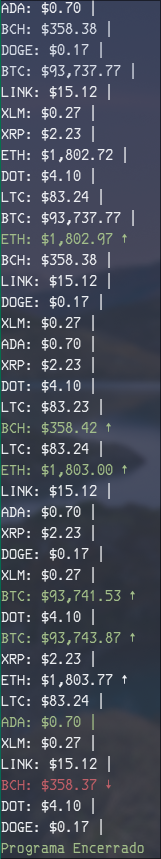
\includegraphics[width=0.2\textwidth]{img1.png}
    \caption{Criptomoedas sendo atualizadas e programa sendo encerrado com Esc}
    \label{fig:img1}
\end{figure}
\section{Conclusão}

Todos os resultados foram alcançados. A criação do Loop para executar Tasks.WhenAll foi crucial, além de entender como usar o \_ para descarte do retorno da função que monitorava o Esc. Utilizar a orientação a objeto para armazenar os valores das criptomoedas foi essencial.

\end{document}
